\documentclass[MiniProjectMain]{subfiles}
\begin{document}

\chapter{Implementation}
The first section of this chapter describes the graphical user interface. 
The following sections contains the Matlab code for the functions implemented. 
This includes in-line comments and is thus not described further. 

Note, the GUI code is not included!

\section{Graphical User Interface}
The graphical user interface has been implemented in Matlab, using the Matlab GUIDE. On Figure \ref{fig:GUI} the start-up screen can be seen. On Figure \ref{fig:GUIrun} the same view is shown, after a complete encoding and decoding has been performed. 

The GUI offers a lot of handles to change the input of the encoding and decoding procedure. These will all be described here:

\begin{itemize}
\item \textbf{n}: The total code length can be adjusted. As default it is set to 15.

\item \textbf{k}: The message length can be adjusted. As default is is set to 7.

\item Message vector: The button 'Generate Message' generates a random message vector with length k. It will be displayed in the field named 'Message'. Additionally it is possible to enter a message manually in the 'Message' field.

\item \textbf{Generator polynomial}: The button 'Generate Polynomial' writes the default polynomial in the field 'Generator polynomial'. The default is: $G(X) = 1 + X^4 + X^6 + X^7 + X^8$. Additionally it is possible to enter another polynomial manually. 

\item \textbf{Code vector}: The button 'Generate Code' encodes the message vector, using the generator polynomial and displays this in the 'Code vector' field.

\item \textbf{Error vector}: The button 'Generate Error' creates a vector of size n with one or two random bits set to '1'. Additionally this could also be entered manually.

\item \textbf{Run the code}: The button 'Run' will calculate the received vector, based on the code vector and the error vector. Further it will attempt to decode this vector. The fields 'Received', 'Buffer', 'Corrected', 'Syndrome', 'Calculated error', 'Tag', and 'Decoder error' will all be updated with the final values.

\item \textbf{Single stepping}: The button 'Single step' will calculate the received vector and process a single step in the Meggit decoder. All fields will be updated after each step. 

\item \textbf{Resetting}: The button 'Reset' clears all the fields use in the Meggit decoder, but not the inputs.

\end{itemize}


A brief description of the GUI outputs fields:
\begin{itemize}
\item \textbf{'Received'}: This field shows the calculated received vector, and its shifting during decoding.

\item \textbf{'Buffer'}: This field shows the buffer register during and after the Meggit decoding.

\item \textbf{'Corrected'}: This field shows the corrected vector after decoding.

\item \textbf{'Syndrome'}: This field shows the syndrome register of the Meggit decoder.

\item \textbf{'Calculated error'}: This field shows where the Meggit decoder has corrected error bits. 

\item \textbf{'Tag'}: This field displays whether the error pattern could be corrected or not.

\item \textbf{'Decoder error'}: This field displays whether the corrected vector is equal to the original code vector or not. 
\end{itemize}

\begin{figure}
\begin{center}
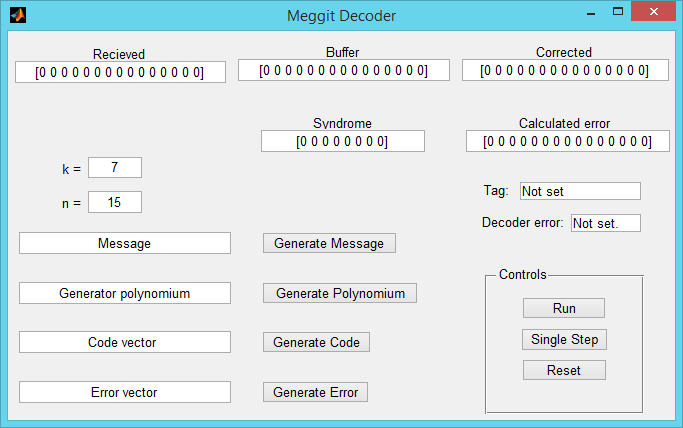
\includegraphics[width=.9\textwidth]{GUI}
\caption{Graphical User Interface on startup.}
\label{fig:GUI}
\end{center}
\end{figure}

\begin{figure}
\begin{center}
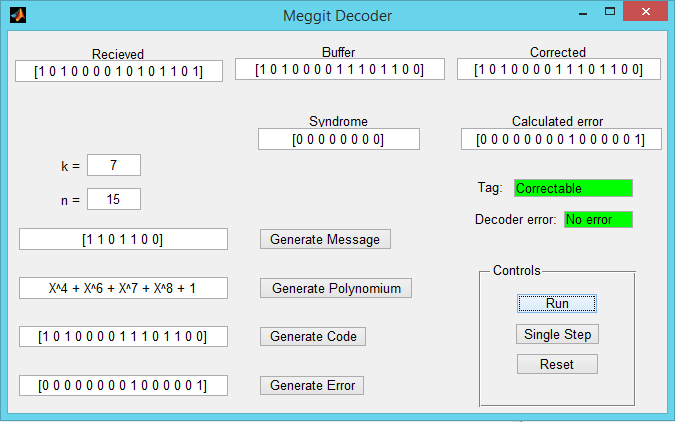
\includegraphics[width=.9\textwidth]{GUIrun}
\caption{Graphical User Interface after a complete run.}
\label{fig:GUIrun}
\end{center}
\end{figure}

\newpage
\section{Encoder}
\begin{lstlisting}[caption=Cyclic encoding]
function [ codeVector ] = cyclicEncode( genPol, messageVector )
% Returns a code vector, given a meassage vector and a cyclic 
% generator polynomial.
% genPol is a generator polynomial in polynomial form.
% messageVector a is in binary form.
% codeVector is the encoded vector in binary for

r = degree(genPol);
k = numel(messageVector);
n = k + r;
% Convert the generator polynomial to vector form.
genVec = pol2polvec(genPol);
% Calculate the generator matrix in systematic form.
[H,G] = cyclgen(n, genVec,'system');
% Encode the meassage vector.
codeVector = rem(messageVector * G,2);
end
\end{lstlisting}

\newpage
\section{Meggit decoder}

\begin{lstlisting}[caption=Cyclic Meggit decoding]
function [ codeVector, errorVector, tag, bufferReg, syndromeReg ] 
= cyclicDecode( receiveVector, genPol, n, k)
% Meggit Decoder

r = degree(genPol);
n1 = numel(receiveVector);
k1 = n1-r;
if(n1 ~= n || k1 ~= k)
   error('The received vector and the generator polynomial does 
   not correspond to the values of n and k'); 
end

% Generator polynomial in vector form:
genVec = pol2polvec(genPol);

% 'Registers' initialization:
bufferReg = zeros(1,n); % Buffer register
codeVector = zeros(1,n); % Corrected output
errorVector = zeros(1,n); % Calculated errors
syndromeReg = zeros(1,r); % Syndrome register
errorDetected = 0; % Error detection 'gate'
tag = 'Not set'; % Correctable/Uncorrectable tag.
% Syndrome vector table used for comparison with the syndromeReg
errSyndTable = generateErrExpr(n, genPol);

for i = 1:n*2
    % Output codeVector shifting
    codeVector = circshift(codeVector,[1 1]);
    % Only output result after the received vector is shifted 
   	% into the buffer.
    if(i > n)
        codeVector(1) = mod(bufferReg(end) + errorDetected,2);
    end

    %Update syndrome register:
    syndromeGate = syndromeReg(end);

    % SyndromeGate feedback and shifting:
    for j = 1:r-1
        syndromeReg(r+1-j) = mod(syndromeReg(r-j) 
        					+ syndromeGate*genVec(r+1-j),2);
    end
    
    % The errorDetected feedback is only used after the buffer 
    % have been filled:
    if(i > n)
        syndromeReg(1) = mod(receiveVector(n) + errorDetected 
        				+ syndromeGate*genVec(1),2);
    else
        syndromeReg(1) = mod(receiveVector(n) 
        				+ syndromeGate*genVec(1),2);
    end
    
    % Compare syndrome register with syndrome vector table:
    for j = 1:n
        if(isequal(errSyndTable(j,:),syndromeReg))
            errorDetected = 1;
            if(i >= n)
                errorVector(2*n-i) = 1;
            end
            break;
        end
        errorDetected = 0;
    end

    % Buffer register shifting and feedback:
    bufferReg = circshift(bufferReg,[1 1]);
    bufferReg(1) = mod(receiveVector(n) + codeVector(1),2);
    
    % Receive vector shifting:
    receiveVector = circshift(receiveVector,[1 1]);
    receiveVector(1) = 0;
end
% Update tag:
if(isequal(syndromeReg,zeros(1,r)))
    tag = 'Correctable';
else
    tag = 'Uncorrectable error';
end
end
\end{lstlisting}

\newpage
\begin{lstlisting}[caption= Generation of error syndrome vectors.]
function [ errSynd ] = generateErrExpr( n, genPol )
% Returns the syndrome vectors, used in a Meggigt decoder for a 
% double-error correcting generator polynomial.
% errSynd = generateErrExpr( n, genPol )

% The degree of the generator polynomial is equal to the length 
% of the syndrome vectors.
r = degree(genPol);
% Convert the generator polynomial to vector representation.
genVec = pol2polvec(genPol); 
% Calculate the parity check matrix in systematic form.
H = cyclgen(n, genVec,'system');
% Possible error vectors used in the Meggit decoder
e = eye(n);
e(:,n) = 1;
%Syndrome vector matrix
errSynd = zeros(n,r);
for i = 1:n
    % syndrome = e*H';
    errSynd(i,:) = mod(e(i,:)*H',2);
end
end
\end{lstlisting}

\newpage
\section{Helper functions}
\begin{lstlisting}[caption=Maximum degree of polynomial]
function d = degree(eq)
% Returns the maximum degree of the input equation.
% d = degree(eq)
% Note: Only accepts an equation with elements with only one '^'.
a = strtrim(strsplit(char(eq),'+'));
d = 0;
for i=1:length(a)
    f = strsplit(char(a(i)),'^');
    if length(f) == 2
        if d < double(sym(f(2)))
            d = double(sym(f(2)));
        end
    end
end
end
\end{lstlisting}

\newpage
\begin{lstlisting}[caption=Convert polynomial to vector form.]
function polvec = pol2polvec(Pol,n)
% Returns the polynomial representation of a symbolic polynomial as a vector.
% The polynomial vector is ascending(left to rigth).
% polvec = pol2polvec(Pol) returns a polynomial vector.
% polvec = pol2polvec(Pol,n) returns a vector of length n, if
% n > length(pol2polvec(Pol))

switch(nargin)
    case 2
        polvec = rot90(sym2poly(Pol),2);
        polvec = [polvec zeros(1,n-length(polvec))];
    case 1
        polvec = rot90(sym2poly(Pol),2);
end
\end{lstlisting}

\end{document}
